% Rapport du projet foot-predictor, version 1 (sous-étape 5.16, jalon J8 ; rapport de cadrage, K.2).
% Compilation : téléverser ce dossier sur Overleaf (pdfLaTeX, puis BibTeX) ; ADR-0034.
% Les chiffres viennent des pages générées de docs/resultats/, des ADR et des retours de session ;
% en cas d'écart, le dépôt fait foi. Équations détaillées : docs/latex/mathematiques/.
\documentclass[11pt,a4paper]{report}

\usepackage[utf8]{inputenc}
\usepackage[T1]{fontenc}
\usepackage{lmodern}
\usepackage[french]{babel}
\usepackage[margin=2.5cm]{geometry}
\usepackage{amsmath,amssymb}
\usepackage{booktabs}
\usepackage{graphicx}
\usepackage{tabularx}
\usepackage[hidelinks]{hyperref}

\newcommand{\code}[1]{\texttt{#1}}

\title{foot-predictor\\[0.5em]\large Prédire la loi du nombre de buts d'un match de football\\[0.3em]
\normalsize Rapport, version 1}
\author{Projet d'apprentissage}
\date{31 octobre 2026 (tag \code{v0.6.0})}

\begin{document}
\maketitle

\begin{abstract}
Ce projet, mené seul à raison d'une dizaine d'heures par semaine, construit une chaîne complète pour
prédire la \emph{loi} du nombre total de buts d'un match des cinq grands championnats européens :
collecte et sauvegarde des données, référentiel reconstruit depuis le brut, variables calculées sans
fuite, protocole d'évaluation figé avant toute mesure, modèles, inférence, API et interface locales.
Le modèle retenu, une régression de Poisson par équipe sur le contexte, un Elo maison et des moyennes
glissantes de buts et de tirs, bat la référence par championnat et par terrain en validation glissante
(\(+0{,}0179\) nat par match, intervalle à 95~\% \([0{,}0133 ; 0{,}0226]\), 7\,156 matchs) et sur un
test scellé de 2\,092 matchs jamais vus (\(+0{,}0189\), \([0{,}0102 ; 0{,}0282]\)), avec une couverture
de son intervalle à 0,2 point de la couverture annoncée. Le marché des paris reste meilleur sur
l'événement \og plus de 2,5 buts \fg{}. L'application prédit en direct les matchs à venir et explique
chaque prédiction ; elle refuse de prédire quand une variable manque.
\end{abstract}

\tableofcontents

% Contexte, objectifs, problématique, contraintes (rapport de cadrage, A et C).

\chapter{Introduction}
\label{chap:introduction}

\section{Contexte}

Le projet est né d'un dépôt existant : un modèle de Poisson qui fonctionnait, une collecte de données
depuis l'API commerciale API-FOOTBALL, une première application. Le rapport de cadrage du 24 septembre
2026 l'a analysé et a recommandé une \emph{refonte ciblée} du cœur de données plutôt qu'une réécriture :
les joueurs étaient identifiés par leur nom, la collecte consommait vingt fois trop de requêtes, le brut
n'était conservé nulle part en dehors d'un volume Docker, et aucun modèle n'était comparé à une
référence naïve. Surtout, l'abonnement payant à l'API expirait trois semaines plus tard : il fallait
d'abord sauvegarder ce qui ne pourrait plus être récupéré gratuitement.

\section{Objectifs}

Le besoin est double. Le produit est une application locale qui liste les matchs d'une date, dit pour
chacun si les données nécessaires sont disponibles, et affiche alors la loi du nombre total de buts :
probabilités de 0, 1, 2\dots{} buts, espérance, intervalle et probabilité de plus de 2,5 buts, avec les
variables utilisées, la version du modèle et la date des données. L'apprentissage est l'autre moitié :
Git, structuration d'un projet Python, bases de données, statistiques inférentielles, modélisation,
tests, API, interface et documentation. Chaque technologie doit répondre à un besoin concret.

\section{Problématique}

Prédire un nombre de buts est un problème très bruité. Si le total \(T\) suit une loi de Poisson de
paramètre \(\lambda \approx 2{,}8\), la variance irréductible vaut 2,8 alors que la variance de
\(\lambda\) d'un match à l'autre n'est que de l'ordre de 0,3 à 0,5 : même un modèle parfait
n'expliquerait qu'environ 10 à 15~\% de la variance. Juger le projet sur l'erreur d'une prédiction
ponctuelle serait donc trompeur. La question devient : \emph{peut-on prédire une loi de probabilité
mieux calibrée et plus informative qu'une référence simple, et mesurer honnêtement ce qu'apporte chaque
information ?} \og Honnêtement \fg{} veut dire ici : variables disponibles avant le match seulement,
protocole fixé avant les mesures, intervalles de confiance sur chaque comparaison, et un ensemble de
test tenu à l'écart jusqu'à la fin.

\section{Contraintes}

\begin{itemize}
  \item \textbf{Temps} : environ 10 heures par semaine, une personne.
  \item \textbf{Argent} : aucun service payant, hormis l'abonnement API-FOOTBALL déjà payé, terminé le
        22 octobre 2026 (ADR-0005).
  \item \textbf{Matériel} : un portable Windows de 3 à 4 ans ; tout tourne en local.
  \item \textbf{Légalité} : seulement des sources dont les conditions le permettent. Transfermarkt est
        écarté par ses conditions d'utilisation, Understat par son \code{robots.txt} (ADR-0023).
\end{itemize}

\section{Démarche}

Le travail est découpé en six parties (collecte, référentiel, variables, modèles, application,
version intermédiaire), chacune en phase A (développement) puis phase B (exécution sur les données
définitives). Chaque décision est consignée dans une \emph{ADR} (Architecture Decision Record) qui ne se
réécrit pas : 46 ADR à ce jour, listées en annexe~\ref{chap:annexes}. Chaque erreur résolue a son entrée
dans un journal (64 entrées). Le code est écrit avec un assistant de programmation (Claude Code), sous
des règles stables (\code{CLAUDE.md}) : une tâche, une branche, une revue de code, une fusion après
intégration continue verte. Le présent rapport résume ; le détail est dans le dépôt.

\section{Plan du rapport}

Le chapitre~\ref{chap:etat-art} situe les modèles et les métriques dans la littérature. Les
chapitres~\ref{chap:donnees} et~\ref{chap:architecture} décrivent les données et l'architecture. Le
chapitre~\ref{chap:methode} présente les variables, le protocole et les modèles, et le
chapitre~\ref{chap:resultats} leurs résultats. Le chapitre~\ref{chap:application} décrit l'inférence,
l'API et l'interface. Le chapitre~\ref{chap:bilan} fait le bilan : critères de réussite, limites,
difficultés et perspectives.

% État de l'art, limité à ce qui éclaire les choix du projet.

\chapter{État de l'art}
\label{chap:etat-art}

\section{Modèles de buts}

\paragraph{Poisson par équipe.} Depuis Maher~\cite{maher1982}, on modélise les buts de chaque équipe
par une loi de Poisson dont le logarithme de la moyenne combine l'attaque de l'équipe, la défense de
l'adversaire et l'avantage du terrain. Les deux comptages sont supposés indépendants sachant ces
forces ; le total suit alors une loi de Poisson de paramètre \(\lambda_{\mathrm{dom}} +
\lambda_{\mathrm{ext}}\).

\paragraph{Dépendance entre équipes.} Dixon et Coles~\cite{dixon1997} corrigent les quatre scores les
plus faibles (0-0, 1-0, 0-1, 1-1) par un paramètre \(\rho\), et pondèrent les matchs anciens par une
décroissance exponentielle. Karlis et Ntzoufras~\cite{karlis2003} proposent un Poisson bivarié, avec
une composante commune aux deux équipes. Ces raffinements visent surtout le score exact ; le projet
mesure s'ils changent la loi du \emph{total} (section~\ref{sec:resultats-modeles}).

\paragraph{Force des équipes.} Le classement Elo~\cite{elo1978}, conçu pour les échecs, met à jour une
note après chaque match selon l'écart entre résultat et attente. Hvattum et Arntzen~\cite{hvattum2010}
montrent qu'une note Elo est une variable efficace pour prédire les résultats en football. Faute de
source gratuite (le service ClubElo est passé derrière une authentification), le projet calcule son
propre Elo.

\paragraph{Dispersion.} La loi de Poisson impose une variance égale à la moyenne. Le test de Cameron
et Trivedi~\cite{cameron1990} détecte une surdispersion, qui justifierait une binomiale négative.

\section{Évaluer une prédiction probabiliste}

Une règle de score \emph{strictement propre} n'est minimisée en espérance que par la vraie loi
\cite{gneiting2007} : elle récompense l'honnêteté de la probabilité annoncée. Le log-loss en est une,
sensible à toute la loi. Le RPS (\emph{ranked probability score}) tient compte de l'ordre des
catégories, ce qui convient aux résultats sportifs~\cite{constantinou2012}. Pour une loi discrète, le
PIT randomisé~\cite{czado2009} vérifie la calibration d'ensemble. Comparer deux modèles sur les mêmes
matchs se fait par la différence de leurs pertes ; le test de Diebold et Mariano~\cite{diebold1995}
en donne la significativité, et le bootstrap par blocs~\cite{kunsch1989} un intervalle de confiance
qui respecte la dépendance entre matchs d'une même journée.

\section{Le marché des paris}

Les cotes agrègent l'information des bookmakers et des parieurs ; Dixon et Coles s'en servaient déjà
pour tester leur modèle~\cite{dixon1997}. Le projet les utilise comme \emph{référence}, jamais comme
variable : un modèle qui lirait les cotes ne prédirait plus le football, mais le marché (ADR-0036).

% Données : sources, collecte, gel, référentiel, qualité, scellé (parties 1 et 2 ; DATA_FREEZE.md).

\chapter{Données}
\label{chap:donnees}

\section{Sources}

\begin{center}
\begin{tabularx}{\textwidth}{lXl}
\toprule
Source & Contenu utilisé & Statut \\
\midrule
API-FOOTBALL & matchs, compositions, statistiques d'équipe et de joueurs, profils, entraîneurs,
               classements, depuis 2015-16 & abonnement terminé le 22/10/2026 \\
football-data & résultats depuis 2000, tirs, cotes plus ou moins 2,5 buts ; résultats et prochains
                matchs en direct & gratuit, deux mises à jour par semaine \\
\bottomrule
\end{tabularx}
\end{center}

Understat (xG) est écarté : son \code{robots.txt} interdit la collecte automatique (ADR-0023). Les xG
d'API-FOOTBALL ne couvrant que les saisons récentes, le projet construit un \code{xg\_proxy} à partir
des tirs cadrés (ADR-0032, ADR-0035).

\section{Collecte et gel}

\paragraph{Brut d'abord.} Chaque réponse de l'API est écrite telle quelle dans un fichier
\code{.json.gz}, avec une ligne dans un journal de requêtes (ADR-0003) ; les CSV de football-data sont
gardés octet pour octet (ADR-0024). Rien n'est jamais modifié dans ce dossier : tout le reste se
reconstruit à partir de lui.

\paragraph{Collecteur v2.} Le collecteur demande les matchs par lots de 20 (un seul appel rend
compositions, événements et statistiques), lit le champ d'erreurs de l'API, reprend après une
interruption et prend un verrou avant toute écriture (ADR-0004, ADR-0018). Le périmètre est collecté
par paliers : top 5 et deuxièmes divisions de 2015-16 à 2026-27, coupes d'Europe et coupes nationales,
autres championnats, classements et profils de joueurs (ADR-0002).

\paragraph{Gel du 19 octobre 2026.} Avant la fin de l'abonnement, le brut est figé (tag
\code{data-freeze-2026-10}) : \textbf{17\,336 fichiers}, 306~Mo compressés, \textbf{102\,554 matchs
terminés}, tous avec leur détail. Le brut est sauvegardé sur un disque externe, puis restauré et
recompté pour vérifier la sauvegarde (ADR-0006). Un journal \og T-60 \fg{} a aussi enregistré, du 9 au
18 octobre, les compositions publiées une heure avant le coup d'envoi, pour la version
intermédiaire (ADR-0017).

\section{Référentiel}

La commande \code{load} reconstruit entièrement le schéma \code{staging} de Postgres à partir du brut :
compétitions, équipes, joueurs, matchs, compositions, tirs et cotes (ADR-0008). Les identifiants sont
ceux d'API-FOOTBALL, jamais les noms : deux joueurs homonymes restent distincts. Les corrections
(équipes de football-data à rapprocher, collisions d'identifiants) sont des fichiers YAML relus par
\code{load}, jamais des modifications à la main dans la base. Sur le brut définitif, \code{load}
produit 167\,980 matchs en un peu plus de 8 minutes. Deux chargements successifs donnent 15 empreintes
de tables sur 15 identiques : la reconstruction est reproductible.

\section{Qualité}

Des contrôles chiffrés accompagnent chaque chargement (\code{check-referentiel}) :

\begin{itemize}
  \item appariement des matchs de football-data et d'API-FOOTBALL : 99,98~\% (seuil : 99,5~\%) ;
  \item identité des joueurs : collisions d'identifiants exclues automatiquement et comptées
        (ADR-0020) ; 0,14~\% des matchs du top 5 touchés par une exclusion (seuil : 1~\%) ;
  \item ruptures de série signalées plutôt que corrigées : les tirs de football-data de la Serie A
        de 2018-19 à 2020-21 ne se comparent pas aux autres saisons (ADR-0029), d'où une source de tirs
        choisie saison par saison (ADR-0035).
\end{itemize}

\section{Le scellé}

Tous les matchs joués à partir du 1\textsuperscript{er} juillet 2025 sont \emph{sous scellés}
(ADR-0012) : aucune de leurs valeurs (score, tirs, cotes) n'a été lue pendant le développement. Ce
n'est pas qu'une consigne : toute lecture des matchs passe par une seule fonction,
\code{features/sources.py}, qui filtre la date en SQL, et des tests d'architecture vérifient
qu'aucun autre module n'interroge la table des matchs (ADR-0028). Le scellé a servi à deux tests, un par
horizon, chacun une seule fois (chapitre~\ref{chap:resultats}). Depuis le premier, l'inférence seule peut
lire les matchs scellés, comme historique de variables (ADR-0045) ; depuis le second, elle peut aussi les
rejouer, avec leur score mais sans leurs cotes (ADR-0052). Le développement ne les lit toujours pas.

\section{Compositions et entraîneurs}

L'horizon H2 (chapitre~\ref{chap:methode}) s'appuie sur des données déjà sauvegardées au gel : pour chaque
match, la feuille de match (onze de départ, remplaçants, entraîneur, formation) et, pour chaque joueur
inscrit, ses minutes, sa note et son poste, avec le profil du joueur (date de naissance). Elles
viennent d'API-FOOTBALL depuis 2015-16 (entraîneurs depuis 2016-17) et sont lues par la même porte unique
que les matchs, qui filtre le scellé en SQL. Aucun \code{load} supplémentaire n'a été nécessaire. Deux
limites en découlent : les notes sont calculées après le match par le fournisseur, selon une formule
inconnue, et seuls les matchs \emph{antérieurs} servent ; et aucune composition n'arrive plus après la fin
de l'abonnement, d'où un horizon H2 de rejeu seulement.

% Architecture : couches, dépôt, outils, garde-fous (rapport de cadrage, F ; ADR-0022, 0025, 0028, 0030, 0040).

\chapter{Architecture}
\label{chap:architecture}

\section{Couches de données}

\begin{center}
\begin{tabular}{lll}
\toprule
Couche & Support & Produite par \\
\midrule
brut & fichiers \code{.json.gz} et CSV, journal & collecteurs \\
référentiel & Postgres, schéma \code{staging} & \code{load} (reconstruit) \\
variables & instantané Parquet versionné, \code{features.dataset\_version} & \code{features build} \\
modèles & fichiers \code{joblib}, cartes d'identité JSON & \code{modeling evaluate}, \code{train} \\
prédictions & Postgres, \code{ops.prediction} & inférence (API, commandes) \\
\bottomrule
\end{tabular}
\end{center}

Chaque couche se reconstruit depuis la précédente par une commande documentée. Le jeu de données est
un instantané : son identifiant (par exemple \code{ds-2026-10-22-bf786ef1}) porte la date et l'empreinte
de son manifeste (chargement lu, commit, paramètres, empreinte de chaque fichier), et une évaluation
cite toujours le jeu qu'elle a lu (ADR-0030).

\section{Code}

Le code Python est un paquet (\code{src/foot\_predictor/}) organisé par étape : \code{collect},
\code{ingestion}, \code{features}, \code{modeling}, \code{inference}, \code{api}, \code{ui}. Les
dépendances sont gérées par \code{uv} ; les migrations de la base par Alembic (8 révisions) ; les deux
bases (travail et test) tournent dans Docker. Les variables sont des \emph{fonctions pures} : elles
reçoivent un historique et rendent des valeurs, sans accès à la base, ce qui les rend testables sur
des données synthétiques. Chaque variable a sa fiche dans un registre (\code{features/registry.yaml}) :
définition, horizon, source.

\section{Garde-fous}

\begin{itemize}
  \item \textbf{Porte unique des données} : toute lecture des matchs passe par
        \code{features/sources.py} ; des tests d'architecture refusent tout autre accès (ADR-0028).
  \item \textbf{Règle temporelle} : une variable d'un match n'utilise que des données strictement
        antérieures au jour du match ; des tests d'\emph{invariance} modifient les matchs postérieurs et
        vérifient que rien ne bouge.
  \item \textbf{Aucun remplissage silencieux} : une valeur incalculable reste vide, et la ligne est
        exclue et comptée, jamais remplie par une moyenne.
  \item \textbf{Protocole figé} : le protocole d'évaluation est écrit et marqué d'un tag Git
        (\code{protocole-v1}) avant toute évaluation de modèle (ADR-0037).
  \item \textbf{Gel avant un test scellé} : la liste du test est figée par un tag (\code{pre-scelle-h1},
        \code{pre-scelle-h2}) ; jusqu'au test, le code d'évaluation et des variables ne change plus, et la
        commande refuse elle-même un code modifié depuis le tag ou un second lancement.
  \item \textbf{Garde du modèle testé} : une commande vérifie que le rejeu reproduit, à
        \(10^{-12}\) près, les prédictions des deux tests scellés (ADR-0052).
  \item \textbf{Secrets et données hors Git} : clés dans des fichiers \code{.env} ignorés, hooks de
        détection de secrets ; aucune donnée ni aucun modèle n'est versionné.
\end{itemize}

\section{Flux de travail}

Git suit un modèle simple (ADR-0022) : une seule branche longue, \code{main}, des branches courtes, une
demande de fusion (PR) par tâche, fusionnée après intégration continue verte (GitHub Actions : ruff et
957 tests), et des tags aux jalons (\code{v0.3.0} à \code{v1.0.0}, puis la version intermédiaire). La documentation suit la même
discipline : un état du projet mis à jour à chaque session, un mode d'emploi par étape, un retour écrit
à la fin de chaque lot de travail.

\section{Application}

L'inférence calcule les variables d'un match par la même fonction que l'entraînement. Une API FastAPI
l'expose en local (\code{127.0.0.1} seulement), et une interface Streamlit l'appelle en HTTP, sans jamais
importer la logique métier ni lire la base (ADR-0040). Le chapitre~\ref{chap:application} la décrit.

% Méthode : cible, variables, protocole, modèles (parties 3 et 4 ; ADR-0009 à 0012, 0031 à 0039).
% Équations détaillées : docs/latex/mathematiques/.

\chapter{Méthode}
\label{chap:methode}

\section{Cible, sortie et horizon}

La cible est le nombre de buts de \emph{chaque équipe} ; la sortie publiée est la loi du \emph{total}
\(T\), repliée sur \(\{0, \dots, 9, \ge 10\}\) (ADR-0009). Modéliser par équipe donne la loi du total
par convolution, et aussi le score exact et le 1N2. L'horizon du MVP, \og H1 \fg{}, est la veille du
match, avant la publication des compositions : seules des informations connues à ce moment entrent dans
les variables (ADR-0010). L'horizon \og H2 \fg{}, une heure avant le coup d'envoi (\og T-60 \fg{}), connaît
en plus le onze de départ et l'entraîneur ; il fait l'objet de la version intermédiaire et se place en
rejeu seulement, faute de compositions après la fin de l'abonnement.

\section{Variables}

Les variables sont regroupées par information, pour mesurer l'apport de chaque groupe :

\begin{center}
\begin{tabularx}{\textwidth}{lX}
\toprule
Groupe & Contenu \\
\midrule
G0, contexte & domicile, championnat, huis clos (périodes sourcées, ADR-0033) \\
G1, force & Elo maison : une échelle par pays, mise à jour par jour, paramètres réglés sur 2005-06 à
            2014-15 puis figés (ADR-0031) \\
G2, production & moyennes glissantes des buts et de l'\code{xg\_proxy}, marqués et encaissés, de
                 l'équipe et de l'adversaire, à décroissance exponentielle en jours et tirées vers la
                 moyenne du championnat (ADR-0032) \\
G3, calendrier & jours de repos, matchs des 14 derniers jours, match européen dans les 4 jours \\
G4, entraîneur (H2) & ancienneté de l'entraîneur dans le club, plafonnée à 365 jours ; indicateur
                      \og nouvel entraîneur \fg{} (moins de 5 matchs) \\
G5, qualité du onze (H2) & note moyenne des 11 titulaires, chaque note étant tirée vers la moyenne de son
                           poste selon le nombre de minutes jouées ; part des \og habituels \fg{}
                           absents ; âge moyen \\
G6, stabilité du onze (H2) & nombre de titulaires communs avec le match précédent ; cohésion par paires
                             pondérée par le rang des matchs ; nouveaux titulaires \\
\bottomrule
\end{tabularx}
\end{center}

L'\code{xg\_proxy} remplace l'xG, absent d'API-FOOTBALL avant 2022-23 : une combinaison des tirs cadrés
et non cadrés, à coefficients positifs ou nuls, estimée une seule fois par moindres carrés sur 2015-16 à
2020-21 (avant tous les plis) puis figée. Le coefficient des tirs non cadrés sort nul :
\(\code{xg\_proxy} = 0{,}3076 \times\) tirs cadrés (ADR-0032, ADR-0035). Sur 2022-23 à 2024-25, sa
corrélation avec l'xG d'API-FOOTBALL valait 0,685 par équipe et par match (première estimation,
ADR-0032). Les moyennes
glissantes ne repartent pas de zéro à chaque saison : l'historique compte sur 730 jours, avec une
demi-vie choisie par validation interne (60, 120 ou 240 jours).

\section{Protocole d'évaluation}

Le protocole est écrit et figé avant toute évaluation (ADR-0037, tag \code{protocole-v1}).

\begin{itemize}
  \item \textbf{Plis} : quatre plis à fenêtre croissante. Pour chaque saison de test, de 2021-22 à
        2024-25, apprentissage sur toutes les saisons antérieures depuis 2015-16, évaluation sur les
        matchs de championnat du top 5 : 7\,156 matchs au total. Les réglages se choisissent par
        validation interne, sur la dernière saison d'apprentissage.
  \item \textbf{Métrique principale} : log-loss de la loi du total ; en complément RPS, Brier de
        \(P(T > 2{,}5)\), calibration par décile, couverture de l'intervalle \([q_{10} ; q_{90}]\).
  \item \textbf{Comparaisons} : sur les mêmes matchs, par différence de log-loss ; intervalle à 95~\%
        par bootstrap par blocs (championnat, saison, journée), 10\,000 rééchantillonnages, graine
        fixe ; test de Diebold-Mariano.
  \item \textbf{Règle de décision} : un modèle plus complexe remplace le plus simple si (i) son gain
        poolé est positif avec un intervalle qui exclut 0, (ii) il gagne dans au moins 3 plis sur 4,
        (iii) sa calibration ne se dégrade pas. Sinon, on garde le plus simple.
  \item \textbf{Essais comptés} : chaque expérience, échecs compris, laisse un rapport ; l'index en
        donne le nombre (17 essais à ce jour, 0 échec).
\end{itemize}

L'intervalle \([q_{10} ; q_{90}]\) d'une loi discrète ne couvre pas exactement 80~\% des matchs : chaque
prédiction publie donc sa \emph{couverture annoncée}, et le critère compare la couverture observée à la
moyenne des couvertures annoncées, à \(\pm 3\) points (ADR-0009).

\section{Modèles}

Les modèles suivent une progression où chaque étape répond à une question (rapport de cadrage, I.4) :

\begin{center}
\begin{tabularx}{\textwidth}{lX}
\toprule
Modèle & Question \\
\midrule
B0 & référence : même loi de Poisson pour tous les matchs \\
B1 & référence : moyennes de buts à domicile et à l'extérieur du championnat \\
M1 & une régression linéaire sur le total suffit-elle ? \\
M2 & une loi de comptage (Poisson sur le total) fait-elle mieux ? \\
M3 & faut-il décomposer par équipe (Poisson par équipe) ? \\
M4 & la loi de Poisson est-elle adéquate, ou faut-il une binomiale négative ? \\
M5 & la dépendance entre les deux équipes (Dixon-Coles) change-t-elle la loi du total ? \\
M6 & plus de variables sous régularisation (ridge, élastique net) ? \\
M7 & un boosting d'arbres à perte de Poisson (H2) fait-il mieux que M3 ? \\
\bottomrule
\end{tabularx}
\end{center}

Le marché des paris (probabilité implicite de plus de 2,5 buts, marge retirée) sert de troisième
référence, sur cet événement seulement ; la cote de clôture, qui intègre les compositions, n'est
qu'une borne haute, jamais une référence de l'horizon H1 (ADR-0036).

\section{Test scellé}

La liste du test est figée avant son lancement, avec le code (tag \code{pre-scelle-h1}, ADR-0039) : le
modèle retenu, B0, B1 et le marché, appris sur 2015-16 à 2024-25, évalués une seule fois sur les matchs
scellés. La commande refuse elle-même un second test et tout code modifié depuis le tag.

\section{L'horizon H2 : méthode}
\label{sec:methode-h2}

La version intermédiaire répond à une question : que rapporte la composition des équipes ? La méthode est
celle de l'horizon H1, avec quatre précautions propres.

\begin{itemize}
  \item \textbf{Spécification avant mesure.} Les variables, les grilles, le chemin de décision et ce qui est
        publié sont écrits dans une ADR \emph{avant} chaque expérience (ADR-0048, ADR-0049). La règle de
        décision du protocole figé s'applique mécaniquement, dans l'ordre stabilité, qualité du onze,
        entraîneur, chaque groupe s'ajoutant au modèle retenu juste avant lui.
  \item \textbf{Même fonction, composition à T-60.} Les variables du match cible n'utilisent que son onze
        et son entraîneur annoncés ; les minutes et les notes de ce match n'existent pas encore. Celles des
        matchs \emph{passés} sont prises à un jour strictement antérieur (ADR-0047). Une valeur incalculable
        reste vide, et la ligne est exclue et comptée.
  \item \textbf{Rodage.} Les notes de 2015-16 n'ont pas d'historique pour être tirées vers la moyenne du
        poste : l'apprentissage de la qualité du onze commence en 2016-17, celui de l'entraîneur en 2017-18,
        et ces lignes de rodage sont comptées, non utilisées.
  \item \textbf{Garde de l'horizon H1.} Aucun modèle H1 ni aucune colonne H1 ne change : une PR qui touche
        aux variables ou aux modèles montre que les prédictions du modèle final H1 et les colonnes H1 du jeu
        sont inchangées (ADR-0044).
\end{itemize}

Les trois groupes s'ajoutent à la structure M3 (Poisson par équipe), comme pour H1. Deux autres structures
sont ensuite comparées à M3 avec les variables retenues : un ridge (M6) et un boosting d'arbres à perte de
Poisson (M7), chacune une fois, sur un chemin de décision écrit d'avance (ADR-0049).

\paragraph{Test scellé de H2.} Le second test réutilise les mêmes matchs scellés, une dernière fois, sur une
liste figée par un tag (\code{pre-scelle-h2}, ADR-0050) : le modèle H1 (référence), le modèle H2 retenu, B1
et le marché. La comparaison de décision est unique : modèle H1 contre modèle H2. Avant l'évaluation, les
colonnes H1 du jeu scellé de H2 doivent être identiques au bit près à celles du premier test ; le nombre de
lignes écartées faute de variables est publié ; un échec technique ne se relance pas sans nouvelle ADR. Les
règles de lecture sont écrites avant le test : un écart non significatif, résultat attendu vu la puissance, ne
retire pas le groupe.

\paragraph{Après le test.} Le rejeu des saisons scellées s'ouvre (ADR-0052) sur trois règles : la condition
est lue dans le journal du scellé, le modèle est celui du test, le score est servi mais pas les cotes. Une
commande de garde vérifie que le rejeu reproduit les prédictions des deux tests à \(10^{-12}\) près. Le
journal des prédictions live fait l'objet d'un relevé \emph{descriptif} : aucune règle de décision, aucun
modèle changé à partir de lui, aucune conclusion avant 8 journées.

% Résultats : références, modèles, ablations, test scellé, marché.
% Chiffres recopiés des pages générées docs/resultats/ (references.md, modeles.md, ablations.md,
% test_scelle_h1.md) ; log-loss en nats par match.

\chapter{Résultats}
\label{chap:resultats}

\section{Références}

Sur les 7\,156 matchs des quatre plis, B0 (même loi pour tous) a un log-loss de 1,9029 et B1 (moyennes
du championnat par terrain) de 1,8984 : connaître le championnat et le terrain fait gagner 0,0046 nat par
match (\([0{,}0010 ; 0{,}0080]\)), soit 0,24~\%. C'est l'ordre de grandeur attendu pour une variable aussi
bruitée. Le marché avant clôture est loin devant sur l'événement plus ou moins 2,5 buts : Brier de 0,2387
contre 0,2478 pour B1 ; la clôture fait encore mieux (0,2374), signe que de l'information arrive jusqu'au
coup d'envoi.

\section{Structures de modèles}
\label{sec:resultats-modeles}

Avec les mêmes variables (G0 et G1), sur les 4 plis :

\begin{center}
\begin{tabular}{lcccl}
\toprule
Modèle & Log-loss & RPS & Brier \(P(T > 2{,}5)\) & Lecture \\
\midrule
B0 & 1,9029 & 0,1320 & 0,2491 & référence \\
B1 & 1,8984 & 0,1313 & 0,2478 & référence à battre \\
M1, linéaire & 1,9092 & 0,1309 & 0,2471 & moins bon que B1 \\
M2, Poisson sur le total & 1,8930 & 0,1305 & 0,2460 & bat B1 \\
M3, Poisson par équipe & 1,8897 & 0,1301 & 0,2450 & \textbf{structure retenue} \\
M5, Dixon-Coles & 1,8897 & 0,1301 & 0,2450 & sans gain \\
\bottomrule
\end{tabular}
\end{center}

\begin{itemize}
  \item \textbf{La forme de la loi compte.} M1 a la bonne moyenne mais une loi normale : il met 2,5~\%
        de sa masse sur des totaux négatifs et sa variance est supposée constante, alors qu'elle croît
        avec la moyenne. Il perd contre B1 (\(-0{,}0108\), \([-0{,}0166 ; -0{,}0049]\)). M2, avec une loi
        de comptage, le bat de 0,0162.
  \item \textbf{Décomposer par équipe paie} : M3 bat M2 de 0,0033 (\([0{,}0014 ; 0{,}0052]\)), dans les
        4 plis, avec les mêmes variables.
  \item \textbf{Ni la dispersion ni la dépendance ne changent la loi du total.} Les buts d'une équipe
        sont même légèrement sous-dispersés une fois les variables connues (\(\hat\varphi \approx
        0{,}98\)) : la binomiale négative (M4) se confond avec Poisson et n'est pas évaluée. Dixon-Coles
        (M5) estime \(\rho \approx -0{,}06\) : il corrige \(P(T = 1)\) mais dépasse sur \(P(T = 0)\), pour
        un log-loss inchangé.
  \item \textbf{La régularisation n'apporte rien} : avec environ 33\,000 lignes pour une trentaine de
        coefficients, le ridge et l'élastique net font jeu égal avec le Poisson non régularisé (M6).
\end{itemize}

\section{Que rapporte chaque information ?}

Sur la structure M3, les groupes de variables s'ajoutent un à un (figure~\ref{fig:apport}) :

\begin{center}
\begin{tabular}{lccc}
\toprule
Étape & Log-loss & Apport de l'étape [IC 95~\%] & Retenu \\
\midrule
G0, contexte & 1,8990 & \(+0{,}0039\) sur B0 & oui \\
+ G1, Elo & 1,8897 & \(+0{,}0094\) \([0{,}0060 ; 0{,}0128]\) & oui \\
+ G2, glissants & 1,8805 & \(+0{,}0092\) \([0{,}0057 ; 0{,}0127]\) & oui \\
+ G3, calendrier & 1,8806 & \(-0{,}0001\) \([-0{,}0004 ; 0{,}0002]\) & non \\
\bottomrule
\end{tabular}
\end{center}

\begin{figure}[ht]
  \centering
  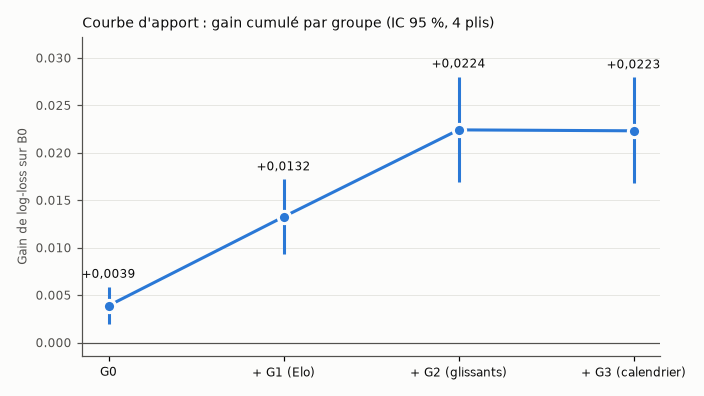
\includegraphics[width=0.75\textwidth]{figures/courbe_apport.png}
  \caption{Gain cumulé de log-loss sur B0 par groupe de variables, avec intervalle à 95~\% (4 plis,
           7\,156 matchs).}
  \label{fig:apport}
\end{figure}

L'Elo dit qui est fort ; les moyennes glissantes disent combien une équipe marque et encaisse, ce qui
est précisément la question du total : elles apportent presque autant que l'Elo. Le calendrier n'apporte
rien. Apprendre aussi sur les deuxièmes divisions ne fait pas mieux que le top 5 seul. Le
\textbf{modèle retenu} (ADR-0039) est donc M3 sur G0, G1 et G2, appris sur le top 5 : il bat B1 de
\(0{,}0179\) (\([0{,}0133 ; 0{,}0226]\)), dans les 4 plis, avec une pente de calibration de 0,95 et une
couverture de son intervalle à \(\pm 1{,}1\) point de l'annoncée.

\section{Test scellé}

Le test a été lancé une fois, sur 2\,092 matchs joués entre le 1\textsuperscript{er} juillet 2025 et le
18 octobre 2026. Un premier lancement a échoué pour une raison technique (une date mal encodée dans le
rapport), sans qu'aucun résultat soit affiché ; la relance unique a été décidée par écrit, avec ses
règles de lecture, puis contrôlée par l'empreinte des prédictions, identique au premier lancement
(ADR-0043).

\begin{center}
\begin{tabular}{lcccc}
\toprule
Modèle & Log-loss & RPS & Brier \(P(T > 2{,}5)\) & Couverture (annoncée) \\
\midrule
Modèle retenu & 1,8805 & 0,1281 & 0,2414 & 87,3~\% (87,5~\%) \\
B1 & 1,8994 & 0,1305 & 0,2457 & 88,3~\% (88,0~\%) \\
B0 & 1,9063 & 0,1316 & 0,2484 & 87,1~\% (87,4~\%) \\
\bottomrule
\end{tabular}
\end{center}

\begin{itemize}
  \item \textbf{Le modèle bat B1} : \(+0{,}0189\) (\([0{,}0102 ; 0{,}0282]\)), un gain du même ordre qu'en
        validation glissante. Il bat aussi B1 en RPS et en Brier.
  \item \textbf{Calibration} : pente de 1,00 ; couverture à 0,2 point de l'annoncée. Par décile de
        \(P(T > 2{,}5)\), l'écart moyen est de 2,5 points, mais la moitié des déciles dépassent 3 points
        (le plus grand : 5,7). Avec 209 matchs par décile, l'erreur d'échantillonnage seule est
        d'environ 3,5 points : ce critère est un diagnostic, publié tel quel (ADR-0037).
  \item \textbf{Le marché reste meilleur} sur l'événement plus ou moins 2,5 buts, sur les 2\,001 matchs
        qui ont une cote : Brier de 0,2418 pour le modèle, 0,2397 pour le marché avant clôture, 0,2383 à
        la clôture. Le modèle comble environ les deux tiers de l'écart entre B1 (0,2458) et le marché.
\end{itemize}

Après le test, aucun modèle H1 n'a été modifié. Le modèle final a été réappris par la même procédure sur
toutes les données, matchs scellés compris : 40\,180 lignes jusqu'au 18 octobre 2026, demi-vie de 240
jours, coefficients à 0,009 au plus de ceux du modèle testé (ADR-0044).

% Application : inférence, disponibilité, live, API, interface, traçabilité (partie 5 ; ADR-0040 à 0046).

\chapter{Application}
\label{chap:application}

\section{Inférence : la même fonction qu'à l'entraînement}

L'inférence n'a aucune formule de variable propre : pour prédire les matchs d'un jour \(J\), elle appelle
la fonction qui construit le jeu d'entraînement sur l'historique arrêté à \(J\), un jour à la fois
(ADR-0040). Sur 17 jours de contrôle, les 622 lignes produites ainsi sont identiques au bit près à celles
du jeu d'entraînement. Deux modes existent :

\begin{itemize}
  \item \textbf{rejeu} : un match passé, prédit par le modèle du pli de sa saison, qui ne l'a jamais vu ;
        les prédictions reproduisent celles de l'évaluation à la précision machine. Les saisons 2021-22 à
        2024-25 sont ouvertes ; les saisons scellées restent fermées jusqu'au test de l'horizon H2
        (ADR-0045) ;
  \item \textbf{live} : un match à venir, prédit par le modèle final, et seulement avant son coup
        d'envoi.
\end{itemize}

\section{Disponibilité}

Pour chaque variable requise, l'inférence dit si elle est \emph{présente}, \emph{manquante} (avec la
raison) ou \emph{périmée} (source en retard). Une seule variable non présente suffit : le match est
\code{unavailable}, et aucune prédiction n'est faite. Aucune valeur de remplacement n'est jamais
utilisée, car une moyenne mise à la place d'une variable absente donnerait une prédiction fausse
présentée avec la même assurance qu'une vraie.

\section{Le live sans abonnement}

Après le gel, le calendrier d'API-FOOTBALL reste figé (dates souvent fausses, aucun résultat). Les
résultats et les prochains matchs de football-data lui sont \emph{superposés en mémoire}, sans rien
écrire dans le référentiel (ADR-0042). L'appariement se fait par championnat, saison et équipes, sans la
date ; un nom inconnu ou une clé ambiguë n'est jamais deviné. Les tirs de football-data remplacent ceux
d'API-FOOTBALL : l'écart de log-loss mesuré est négligeable (\(-0{,}00002\), \([-0{,}00021 ; 0{,}00018]\),
ADR-0041).

\paragraph{Fraîcheur.} football-data publie les résultats environ deux fois par semaine. Avec la règle
d'origine (un championnat entièrement à jour), 91~\% des matchs des sept jours suivants étaient
indisponibles lors du premier live, le 22 octobre. La règle a été révisée après mesure (ADR-0046) : un
match n'attend plus que les résultats de ses deux équipes. L'Elo reste exact ; les moyennes glissantes
deviennent approchées, à moins de 0,0011 près sur \(\lambda\) d'après une répétition sur 2023-24. La part
d'indisponibles est tombée à 14~\%, puis à 10~\% le 31 octobre.

\section{API et interface}

L'API FastAPI (7 routes) liste les matchs d'une date avec leur disponibilité, calcule et trace une
prédiction, décrit le modèle actif et la fraîcheur des données. Elle n'écoute que sur \code{127.0.0.1}
et refuse toute date scellée (code 403). L'interface Streamlit a trois écrans :

\begin{itemize}
  \item \textbf{Matchs} : mode (rejeu ou live), date, championnats ; une pastille de disponibilité par
        match, avec sa raison ; un bouton \og Prédiction \fg{} actif seulement si le match est
        disponible ;
  \item \textbf{Détail} : loi du total en barres, \(E[T]\), \(\lambda\) de chaque équipe, \(P(T > 2{,}5)\),
        intervalle et couverture annoncée, variables utilisées, version du modèle et des données, score
        réel en rejeu, référence de marché en live ;
  \item \textbf{Modèle} : carte d'identité, métriques de validation, courbe d'apport, fraîcheur.
\end{itemize}

L'interface ne parle qu'à l'API, en HTTP : un test d'architecture lui interdit d'importer la logique
métier ou la base.

\section{Traçabilité et journal prospectif}

Chaque prédiction créée est écrite dans \code{ops.prediction} avec tout ce qui a servi à la faire :
modèle, version des données, variables, loi, intervalle, date de complétude des sources. L'écriture est
idempotente : une seconde demande renvoie la ligne existante. En live, une prédiction n'est acceptée
qu'avant le coup d'envoi, et une réponse indisponible n'est jamais écrite. Au 31 octobre 2026, 89
prédictions live sont tracées. Ce journal prospectif servira à évaluer le modèle sur des matchs
réellement futurs ; il n'est pas encore évalué, car lire leurs scores reviendrait à ouvrir le scellé au
développement (ADR-0045).

\section{Tests de bout en bout}

Un test automatisé, en intégration continue, parcourt toute la chaîne sur une petite ligue synthétique :
brut, \code{load}, porte des données, inférence, API, interface, ligne dans \code{ops.prediction}. Sur
les vraies données, la même chaîne a été vérifiée en rejeu et en live le 31 octobre 2026 : l'écran
\og Matchs \fg{} s'affiche en 12 à 17 secondes à froid et en moins d'une demi-seconde ensuite, une
prédiction en 2 à 5 secondes.

% Bilan : critères E.1, limites, difficultés, perspectives, conclusion
% (docs/retours/partie-5-lot4_2026-10-31.md ; JOURNAL_ERREURS.md).

\chapter{Bilan}
\label{chap:bilan}

\section{Critères de réussite du MVP}

Le rapport de cadrage (E.1) fixait six critères ; certains ont été reformulés par des ADR avant toute
mesure.

\begin{center}
\begin{tabularx}{\textwidth}{Xll}
\toprule
Critère & État & Preuve \\
\midrule
1. Tout se reconstruit depuis le brut par des commandes documentées & rempli & 2 chargements identiques \\
2. Le modèle bat B1, intervalle à 95~\% qui exclut 0 & rempli & validation et test scellé \\
3. Calibration de \(P(T > 2{,}5)\) à \(\pm 3\) points par décile & diagnostic & ADR-0037 \\
4. Couverture de l'intervalle à \(\pm 3\) points de l'annoncée & rempli & 0,2 point au test \\
5. Base, API et interface démarrent ; une prédiction s'affiche & rempli & rejeu et live réels \\
6. Documentation et chapitres mathématiques & rempli & ce rapport, docs/ \\
\bottomrule
\end{tabularx}
\end{center}

Le critère 3 n'est pas tenu à la lettre au test scellé (5 déciles sur 10 au-delà de 3 points), alors que
la pente vaut 1,00 : avec environ 209 matchs par décile, 3 points sont sous l'erreur d'échantillonnage.
Le protocole l'avait classé en diagnostic avant toute évaluation ; il est publié tel quel.

\section{Critères de la version intermédiaire}
\label{sec:criteres-e2}

La version intermédiaire (jalon J9) répond à la question \og que rapporte vraiment la composition des
équipes ? \fg{}. Le rapport de cadrage (E.2) fixait ses critères.

\begin{center}
\begin{tabularx}{\textwidth}{Xll}
\toprule
Critère & État & Preuve \\
\midrule
Chaque groupe de variables a un apport mesuré, gain et intervalle, publié & rempli & tableau des
  ablations, chap.~\ref{chap:resultats} \\
Décision argumentée sur la stabilité du onze & rempli & abandonnée pour H2 \\
Régularisation et boosting essayés & rempli & aucune ne remplace M3 \\
Second horizon avec composition, comparé au premier, avec page d'apport & rempli en rejeu & H1 et H2 côte
  à côte, page d'apport \\
Test scellé de l'horizon H2, une seule fois & rempli & non significatif, comme annoncé \\
Prédictions live tracées avant le coup d'envoi pendant au moins 8 journées & en cours (7 sur 8) & 89
  prédictions, premier relevé \\
\bottomrule
\end{tabularx}
\end{center}

Deux éléments prévus par E.2 ne sont pas faits : les services conteneurisés (Compose) et la planification
des collectes, laissés en option par l'ADR-0047. La collecte de l'API est terminée et toute tâche planifiée
passerait par une ADR. Le critère des 8 journées dépend du calendrier : il manque une journée de matchs
tracée avant le coup d'envoi.

\section{Limites}

\begin{itemize}
  \item \textbf{Un second horizon de rejeu seulement.} Avec la composition, H2 n'a pas de live : aucune
        composition n'arrive plus après la fin de l'abonnement, et l'application répond \og indisponible
        \fg{}. Il explique ce que la composition change, il ne prédit pas l'avenir.
  \item \textbf{Un gain de composition minuscule et fragile} : \(0{,}0008\) nat par match, borne basse de
        l'intervalle à \(+0{,}00003\), plus faible à fenêtre égale, concentré en début de saison. Le test
        scellé de H2 ne peut pas le distinguer de zéro (puissance de l'ordre de \(0{,}007\)). Une part de
        l'information de la composition est déjà dans l'Elo (corrélation 0,83 avec la qualité du onze).
  \item \textbf{Des variables de composition imparfaites} : notes calculées après le match par le
        fournisseur, selon une formule inconnue ; les blessures ne sont pas modélisées (un absent connu
        seulement par son absence du onze) ; une variable de G5, surtout l'âge moyen faute de date de
        naissance, manque pour 8~\% des matchs du test.
  \item \textbf{Un seul pli scellé}, d'une saison et quart, utilisé pour deux tests successifs : le résultat
        vaut pour cette période et ces cinq championnats, et l'intervalle de H2 est large (1\,923 matchs).
  \item \textbf{Approximations du live} : moyennes glissantes approchées quand le championnat n'est pas à
        jour (dans une tolérance vérifiée), tirs de football-data à la place de ceux de l'API.
  \item \textbf{Journal prospectif encore court} : 89 prédictions, 7 journées, 48 résultats sur 4 jours ;
        le premier relevé ne conclut pas, par règle.
\end{itemize}

\section{Difficultés}

Le journal compte 68 entrées. Quelques-unes ont changé la méthode :

\begin{itemize}
  \item \textbf{Le premier lancement du test scellé a échoué} (E-059) : une date de l'expérience, lue
        comme un objet date, a fait planter l'écriture du rapport. Aucun résultat n'avait été produit ;
        la relance unique a été décidée par écrit, avec ses règles de lecture, avant d'être lancée.
        Leçon : une commande qui ne s'exécute qu'une fois se répète d'abord de bout en bout, sur son
        vrai fichier d'entrée, avec des données synthétiques.
  \item \textbf{Une exactitude affirmée sans test} (E-063) : la première version de la fraîcheur par
        équipe se disait exacte ; les tests ont montré que l'a priori des moyennes glissantes dépend de
        tout le championnat. La décision a été reprise sur une mesure, avant la fusion.
  \item \textbf{Des identifiants internes instables} (E-058) : ils changent quand le brut grandit. Hors du
        référentiel, on rapproche par l'identifiant de l'API.
  \item \textbf{Un test scellé qui n'aurait pas pu s'exécuter} (E-067) : en relisant la procédure avant de
        poser le tag de gel de H2, on a vu que la construction du jeu scellé, qui vit dans le code gelé,
        était refusée jusqu'au test. Corrigé avant le tag, avec la décision écrite. Leçon : avant de poser un
        gel, parcourir \emph{toutes} les commandes de la phase qu'il protège, pas seulement l'évaluation.
  \item \textbf{Une garde qui n'en était pas une} : une fois le test passé, rien ne protégeait plus le modèle
        H2 testé, le gel étant levé. Une garde chiffrée a été ajoutée avant l'ouverture du rejeu : le rejeu
        doit reproduire les prédictions des tests (ADR-0052).
  \item \textbf{Les rapports d'expérience de 700 Ko} (E-066) : refusés par le hook des gros fichiers, ce qui
        a laissé un lancement noté \og arbre non propre \fg{} ; refait sur arbre propre, les deux conservés.
  \item \textbf{L'outillage} : intégration continue fusionnée avant la fin de ses tests (E-047), échec de
        test masqué par un tube (E-048), formatage des blocs de code des fichiers Markdown (E-049).
        Chacun a laissé une règle écrite.
\end{itemize}

\section{Perspectives}

\begin{itemize}
  \item \textbf{Huitième journée et suivantes} : poursuivre les prédictions live avant le coup d'envoi,
        refaire le relevé après chaque collecte de résultats, et n'en tirer une conclusion qu'à partir de
        8 journées.
  \item \textbf{Un live pour H2} supposerait un réabonnement ou une autre source de compositions : hors
        périmètre aujourd'hui.
  \item \textbf{Blessures} : hors du périmètre de la version intermédiaire (ADR-0047) ; la composition
        annoncée n'en voit que l'effet, par l'absence d'un joueur du onze.
  \item \textbf{Exploitation} : services conteneurisés et collecte live planifiée, laissés en option ; une
        planification de collecte passerait par sa propre ADR.
  \item \textbf{Suivi de la calibration dans le temps}, version avancée du cadrage.
\end{itemize}

\section{Conclusion}

Le MVP est atteint : une chaîne complète, reproductible depuis le brut, qui prédit une loi du nombre de
buts mieux que la référence par championnat et par terrain, sur des matchs jamais vus, avec une
incertitude annoncée qui tient ses promesses. Le gain est petit en valeur absolue (0,019 nat par match),
comme le laissait prévoir le bruit du problème, mais il est mesuré avec un intervalle et confirmé hors
échantillon. Les choix qui ont le plus compté ne sont pas des modèles : sauvegarder le brut avant la fin
de l'abonnement, figer le protocole avant de mesurer, tenir un ensemble de test sous scellés, et refuser
de prédire plutôt que d'inventer une valeur.

La version intermédiaire tient ces mêmes engagements sur une question plus étroite : que rapporte la
composition des équipes ? Réponse mesurée, avec ses intervalles : presque rien. La qualité du onze apporte
un gain de \(0{,}0008\) nat par match, de justesse, fragile et en grande partie déjà dans l'Elo ; la
stabilité du onze et l'entraîneur n'apportent rien ; ni la régularisation ni le boosting ne battent le
Poisson par équipe ; le test scellé de ce second horizon, mené une seule fois, a le même signe sans être
significatif, comme son calcul de puissance l'annonçait. Un résultat aussi modeste, publié tel quel après
des règles écrites avant de regarder, vaut mieux qu'un gain apparent obtenu en cherchant : c'est ce que le
protocole est fait pour garantir.


\appendix
% Annexes : ADR, commandes, glossaire (docs/decisions/README.md, CLAUDE.md).

\chapter{Annexes}
\label{chap:annexes}

\section{Décisions (ADR)}

Titres abrégés ; texte complet dans \code{docs/decisions/}.

{\small
\begin{center}
\begin{tabularx}{\textwidth}{lX}
\toprule
ADR & Décision \\
\midrule
0001--0007 & arrêt de l'ancienne collecte ; périmètre par paliers ; brut en fichiers et journal ; collecteur v2 ;
             fin de l'abonnement et gel ; sauvegarde sur disque externe ; paquet \code{collect} \\
0008 & API-FOOTBALL fait foi pour les identifiants ; \code{staging} reconstruit depuis le brut \\
0009 & cible : buts par équipe ; sortie : loi du total ; métrique : log-loss du total \\
0010--0011 & deux horizons (avant et avec composition) ; après l'abonnement, rejeu et live partiel \\
0012 & validation glissante 2021-22 à 2024-25 ; matchs depuis le 1\textsuperscript{er} juillet 2025 sous scellés \\
0013 & pas de masse salariale ; valeur marchande maison gelée \\
0014 & restructuration de la documentation \\
0015--0016, 0020 & collisions d'identifiants de joueurs ; profils ciblés \\
0017--0019, 0021 & journal T-60 ; verrou de collecte et tâches planifiées ; palier P4 ; code du gel \\
0022 & workflow Git : \code{main}, branches courtes, PR, tags, hooks \\
0023--0024 & football-data retenu, Understat écarté ; bruts externes séparés \\
0025--0026 & bases (travail, test, ancienne base intacte) ; environnement Windows \\
0027 & périmètre des chargeurs du référentiel \\
0028 & scellé technique : porte unique de lecture des matchs \\
0029, 0035 & tirs de football-data ; source des tirs de l'\code{xg\_proxy} \\
0030 & jeu de données versionné, registre des variables \\
0031--0033 & Elo maison ; glissants et \code{xg\_proxy} ; calendrier et huis clos \\
0034 & notebooks sans sorties ; LaTeX compilé sur Overleaf \\
0036 & cotes : référence de marché, jamais une variable \\
0037 & protocole d'évaluation et règle de décision, figés (\code{protocole-v1}) \\
0038--0039 & structure : Poisson par équipe ; modèle MVP H1 et liste du test scellé \\
0040 & inférence, API et interface : même fonction, disponibilité, traçabilité \\
0041--0042 & tirs de football-data en live ; football-data superposé en mémoire \\
0043--0044 & relance unique du test scellé ; modèle final H1 \\
0045--0046 & ouverture du scellé à l'inférence ; fraîcheur par équipe \\
\bottomrule
\end{tabularx}
\end{center}
}

\section{Commandes principales}

{\small
\begin{verbatim}
uv sync --all-groups                                   # environnement
docker compose up -d                                   # bases Postgres
uv run alembic upgrade head                            # migrations
uv run python -m foot_predictor.ingestion load ...     # référentiel depuis le brut
uv run python -m foot_predictor.features build         # jeu de données versionné
uv run python -m foot_predictor.modeling evaluate experiments/<nom>.yaml
uv run python -m foot_predictor.inference live --days 7 --save
uv run python -m foot_predictor.api serve              # API locale
uv run streamlit run src/foot_predictor/ui/app.py      # interface
uv run pytest -q                                       # tests
\end{verbatim}
}

\section{Glossaire}

\begin{description}
  \item[ADR] fiche de décision : contexte, options, choix, conséquences ; jamais réécrite.
  \item[B0, B1] références : même loi pour tous ; moyennes du championnat par terrain.
  \item[Brut] réponses des sources gardées telles quelles, jamais modifiées.
  \item[Couverture annoncée] probabilité, selon le modèle, que le total tombe dans l'intervalle publié.
  \item[H1, H2] horizons de prédiction : avant et avec composition.
  \item[Log-loss] \(-\log\) de la probabilité donnée au total observé ; plus petit est meilleur.
  \item[Pli] découpage apprentissage puis test sur une saison future.
  \item[Rejeu] prédiction d'un match passé par un modèle qui ne l'a jamais vu.
  \item[Scellé] matchs tenus à l'écart du développement, pour un test unique.
  \item[\code{staging}] référentiel en base, reconstruit depuis le brut.
\end{description}


\bibliographystyle{plain}
\bibliography{references}

\end{document}
